\documentclass[a4paper,12pt]{article}
\usepackage[T1]{fontenc}
\usepackage{ninecolors}
\usepackage{booktabs}
\usepackage{caption}
\usepackage{tabularray}
\usepackage{hyperref}
\usepackage{graphicx}
\usepackage{subcaption}
\usepackage{parskip}
\usepackage{tikz}
\usepackage{circuitikz}
\usepackage[tocentry]{vhistory}
\usepackage{float}
\hypersetup{
  colorlinks=true,
  linkcolor=blue,
  filecolor=magenta,
  urlcolor=cyan,
  pdftitle={Hypno},
  pdfpagemode=FullScreen,
}
\graphicspath{ {img/} }
\captionsetup[table]{position=bottom}
\usepackage{geometry}
\usepackage{siunitx}
\usepackage{awesomebox}

\tikzset{
  padStyle/.style={line width=1mm, draw=orange, fill=none}
}

\tikzset{
  partStyle/.style={line width=1mm, draw=black, fill=none, rounded corners=4pt}
}

\begin{document}

\begin{titlepage}
  \vspace*{\stretch{1.0}}
  \begin{center}
    \Large\textbf{Hypno}\\
    \large{Delay Kit by Pedal Markt}
  \end{center}
  \vspace*{\fill}
  \begin{center}
    \vhCurrentDate\\
    { Rev}\vhCurrentVersion
  \end{center}
\end{titlepage}

\tableofcontents
\pagebreak

\section{Introduction}

TODO

Enclosures for Hypno and other pedals in the Beastly Series
were designed by \href{https://fiz.gallery/}{Agata Fiz.}

\begin{figure}[h!]
  \centering
  \begin{subfigure}[b]{0.49\textwidth}
    \centering
    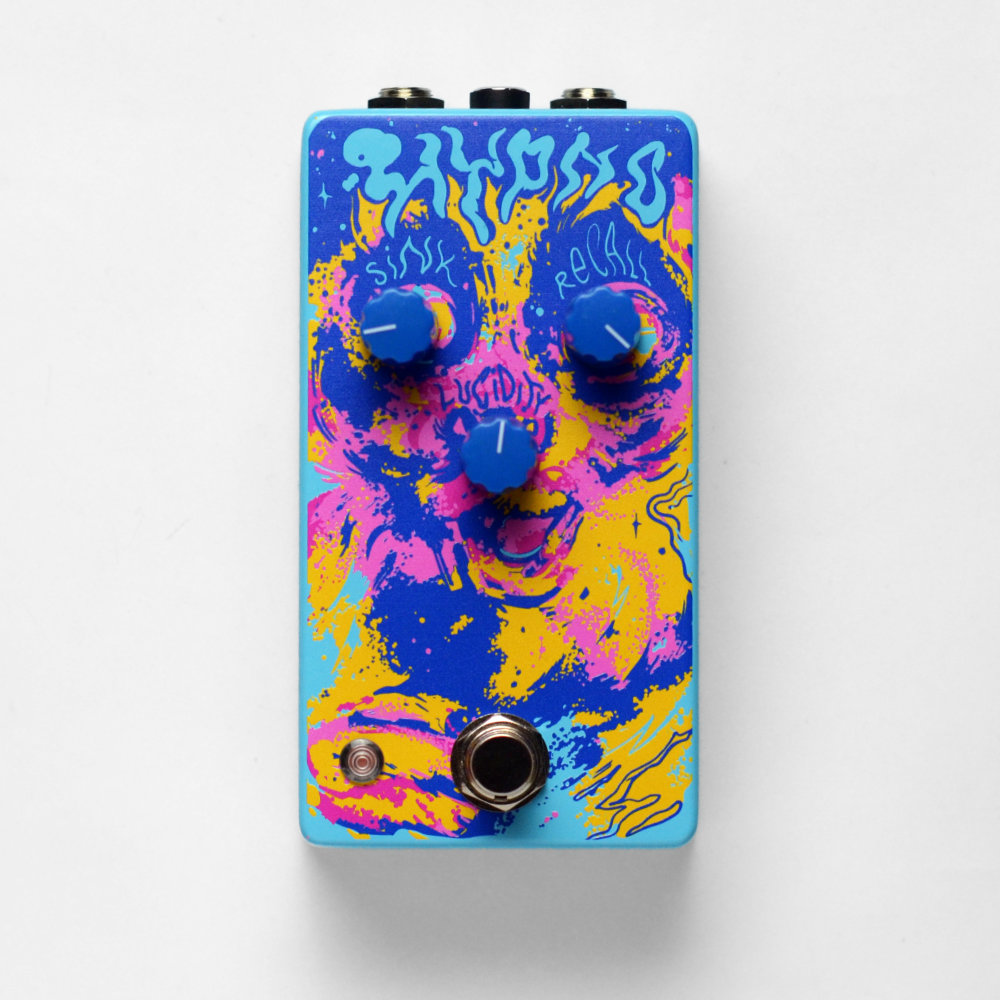
\includegraphics[width=\textwidth]{hypno-outside-1000px.jpg}
  \end{subfigure}
  \begin{subfigure}[b]{0.49\textwidth}
    \centering
    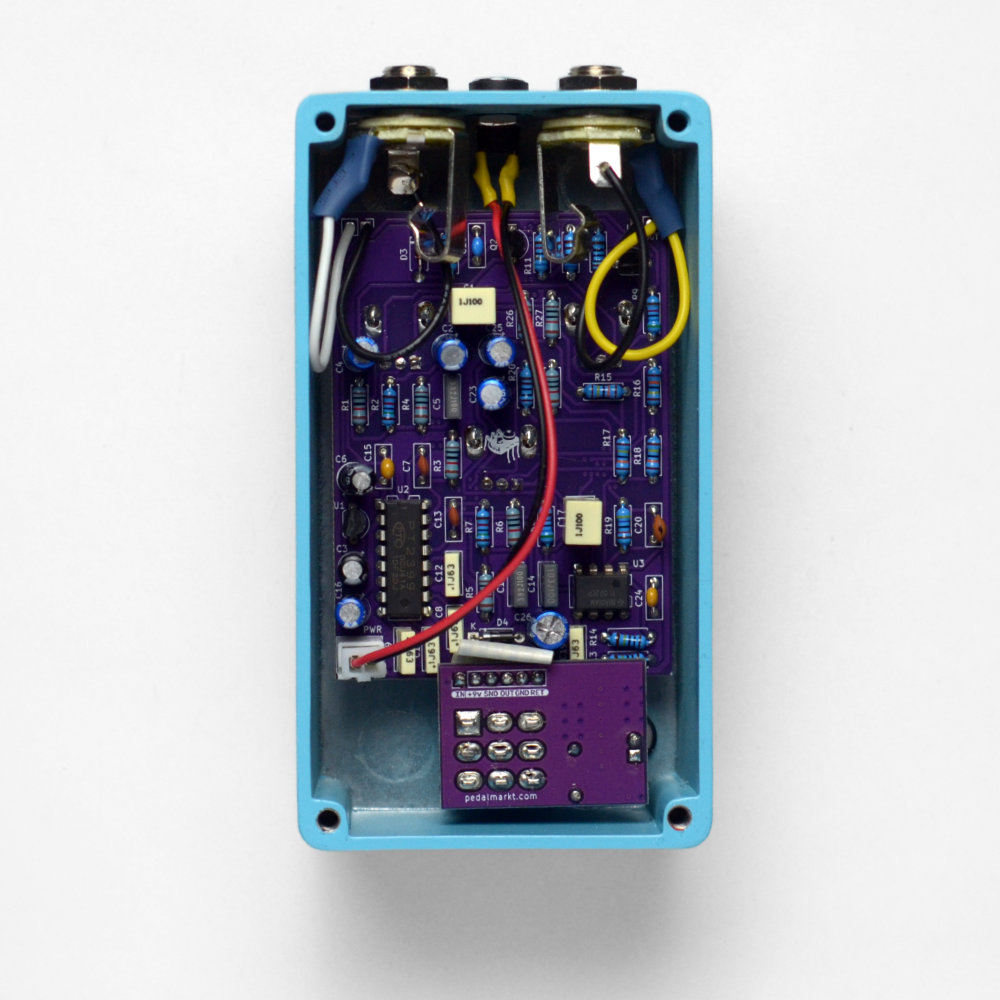
\includegraphics[width=\textwidth]{hypno-inside-1000px.jpg}
  \end{subfigure}
  \caption{Hypno: oustide and inside}
  \label{fig:Hypno}
\end{figure}


\pagebreak

\section{BOM – Bill of Materials}

BOM is a document that lists the parts you'd need to build a
project. Each row corresponds to a component with a certain
value, for example, a `ceramic capacitor with value 1nF.`
There could be one or more actual physical parts per
row, their designators are listed in the \textit{Reference}
column.

% \tipbox{
%   Components in the BOM are listed in order of assembly. Go
%   through the table top to bottom. If you haven't built a
%   kit before, check out the
%   \hyperref[sec:steps]{Step-by-step Instructions} first.
% }

\tipbox{
  In the BOM \textit{text in italic font} gives tips about how to mount or
  solder parts.
}

\newgeometry{hmargin={1cm}}

\begin{longtblr}[caption = {BOM}]{
  hlines,
  vlines,
  rows={ht=1.2em},
  row{even}={bg=gray9},
  row{1}={bg=gray3,fg=white},
  width=\linewidth,
  colspec={lX[1]llX[2]},
}
  \hspace{1em}
  & \textbf{Ref}
  & \textbf{Value}
  & \textbf{Qnty}
  & \textbf{Description}
  \\
  \SetCell[c=5]{c,bg=gray6,fg=white}\textbf{Outboard}
  \\
  \hspace{1em}
  & – & Enclosure & 1 & \textit{Mount the DC
  jack, Footswitch and Lampshade into the enclosure
  before soldering}
  \\
  \hspace{1em}
  & -- & Lampshade & 1
  & Small transparent plastic part for the LED,
  \textit{mount in enclosure before putting the boards in}
  \\
  \hspace{1em}
  & -- & Rubber Ring & 1
  & \textit{Use it to keep Lampshade in place}
  \\
  \hspace{1em}
  & -- & DC Jack & 1
  & Black plastic part with a nut, \textit{mount in
  enclosure before soldering}
  \\
  \hspace{1em}
  & -- & DC Cable & 1
  & Red and black cables in a JST connector, \textit{cut to
  $\approx10cm$ and solder to DC Jack once it's mounted in
  enclosure. Black wire to shorter lug, red to the longer
  one.}
  \\
  \hspace{1em}
  & -- & Audio Jack & 2 & \textit{Only mount these in the
  enclosure together with the main board once they are wired up}
  \\
  \SetCell[c=5]{c,bg=gray6,fg=white}\textbf{Main board, floor side}
  \\
  \hspace{1em}
  & GND & Wire & 2 & $\approx5cm$, black, \textit{strip and
  tin the ends}
  \\
  \hspace{1em}
  & IN & Wire & 1 & $\approx5cm$, any color, \textit{strip and tin
  the ends}
  \\
  \hspace{1em}
  & OUT & Wire & 1 & $\approx5cm$, any other color,
  \textit{strip and tin the ends}
  \\
  \hspace{1em}
  & R8 & 5.6k & 1
  & Resistor
  \\
  \hspace{1em}
  & R9 & 56k & 1 & Resistor
  \\
  \hspace{1em}
  & R10 & 100 & 1 & Resistor
  \\
  \hspace{1em}
  & R11 & 68k & 1 & Resistor
  \\
  \hspace{1em}
  & R12 & 100k & 1 & Resistor
  \\
  \hspace{1em}
  & R19 & 470k & 1 & Resistor
  \\
  \hspace{1em}
  & R20 & 1k & 1 & Resistor
  \\
  \hspace{1em}
  & R21 & 6.8k & 1 & Resistor
  \\
  \hspace{1em}
  & R2, R7 & 15k & 2 & Resistor
  \\
  \hspace{1em}
  & R13, R14 & 1M & 2 & Resistor
  \\
  \hspace{1em}
  & R15, R16, R17, R18 & 140k & 4 & Resistor
  \\
  \hspace{1em}
  & R1, R3, R4, R5, R6, R25, R26, R27 & 10k & 8 & Resistor
  \\
  \hspace{1em} & U2 & PT2399 & 1 & Delay chip. \textit{Please
  use socket. Orientation matters}
  \\
  \hspace{1em} & U3 & TL072 & 1 & Dual opamp. \textit{Please
  use socket. Orientation matters}
  \\
  \hspace{1em}
  & C18 & 1u & 1
  & Ceramic capacitor
  \\
  \hspace{1em}
  & C20 & 2.2p & 1
  & Ceramic capacitor
  \\
  \hspace{1em}
  & C7, C13 & 560p & 2
  & Ceramic capacitor
  \\
  \hspace{1em}
  & C15, C24 & 100n & 2
  & Ceramic capacitor
  \\
  \hspace{1em}
  & J1 & Power Socket & 1
  & JST 2-pin m, in the bottom-left part of the board,
  \textit{orientation matters}
  \\
  \hspace{1em}
  & Q1, Q2 & 2N3904 & 2
  & NPN transistor, \textit{orientation matters}
  \\
  \hspace{1em}
  & U1 & L78L05 & 1
  & Voltage regulator, \textit{orientation matters}
  \\
  \hspace{1em}
  & C14 & 10n & 1
  & Film capacitor
  \\
  \hspace{1em}
  & C5, C11 & 3.9n & 2
  & Film capacitor
  \\
  \hspace{1em}
  & C8, C9, C10, C12, C19 & 100n & 5
  & Film capacitor
  \\
  \hspace{1em}
  & C1, C17 & 1u & 2
  & Film capacitor
  \\
  \hspace{1em}
  & C6 & 100n & 1
  & Electrolytic capacitor, \textit{orientation matters}
  \\
  \hspace{1em}
  & C3 & 330n & 1
  & Electrolytic capacitor, \textit{orientation matters}
  \\
  \hspace{1em}
  & C26 & 100u & 1
  & Electrolytic capacitor, \textit{orientation matters}
  \\
  \hspace{1em}
  & C16, C25 & 10u & 2
  & Electrolytic capacitor, \textit{orientation matters}
  \\
  \hspace{1em}
  & C2, C4, C23 & 4.7u & 3
  & Electrolytic capacitor, \textit{orientation matters}
  \\
  \SetCell[c=5]{c,bg=gray6,fg=white}\textbf{Main board, player side}
  \\
  \hspace{1em}
  & -- & Ribbon cable & 1
  & Pads for that cable are in the bottom-center of the main
  board, \textit{solder one end to main board, another to
  switch board, \textbf{make sure pin names on the two
  boards match, IN on one board is connected to IN on the
  other board etc}}
  \\
  \hspace{1em}
  & RV1 (Sink) & C10k & 1
  & Potentiometer
  \\
  \hspace{1em}
  & RV2 (Recall) & A100k & 1
  & Potentiometer
  \\
  \hspace{1em}
  & RV3 (Lucidity) & B100k & 1
  & Potentiometer
  \\
  \SetCell[c=5]{c,bg=gray6,fg=white}\textbf{Switch board, player side}
  \\
  \hspace{1em}
  & Rled & 1k & 1
  & \textit{larger value will make the LED
  dimmer, values up to 6.8k are reasonable}
  \\
  \hspace{1em}
  & -- & LED & 1
  & \textit{Insert in PCB first. Solder last, once the
  main board is in the enclosure. Orientation matters}
  \\
  \hspace{1em}
  & -- & Footswitch & 1
  & \textit{Mount in enclosure before putting the boards in}
  \\
\end{longtblr}

\restoregeometry{}

\subsection{Note on values}

Different kits and schematics designate values differently.
For example, these usually mean the same value:
\\
$\SI{2.2}{\kohm} = 2.2k = 2k2 = 2.2 \times 10^{3} Ohm = 2200Ohm$
\\
$\SI{4.7}{\uF} = 4.7u = 4u7 = 4.7 \times 10^{-6} Farad = 0.0000047 Farad$

\begin{table}[h!]
  \caption{Component values}
  \centerline{
    \begin{tblr}{
      hlines,
      vlines,
      rows={ht=1.2em},
      row{1}={bg=gray3,fg=white},
      colspec={Xrr}
    }
      \textbf{Value}
      & \textbf{Multiplier}
      & \textbf{Unit}
      \\
      \SetCell[c=3]{c}\textbf{Resistance}
      \\
      \SI{100}{\ohm}, 100R, 100 & 1 & Ohm
      \\
      \SI{1}{\kohm}, 1k & $10^{3}$ & Ohm
      \\
      \SI{1}{\Mohm}, 1M & $10^{6}$ & Ohm
      \\
      \SetCell[c=3]{c}\textbf{Capacitance}
      \\
      \SI{1}{\pF}, 1p & $10^{-12}$ & Farad
      \\
      \SI{1}{\nF}, 1n & $10^{-9}$ & Farad
      \\
      \SI{1}{\uF}, 1u & $10^{-6}$ & Farad
    \end{tblr}
  }
\end{table}

\pagebreak

\section{Transistors}
\label{sec:transistors}

The circuit consists of just a handful of parts. Transistor
selection and bias play a huge role in the sound of the
pedal.

The stock transistors we use for Fur Face are BC108, Q1
biased to about \SI{1.3}{\V}, Q2 to about \SI{5.8}{\V}.

If you'd like to try out and hear different transistors, the
best way is to solder sockets in place of Q1 and Q2 on the
PCB. Swap transistors in those sockets without soldering
them.

When inserting the transistors, please match their pinout to
the expected pinout indicated on the PCB: E to emitter, B to
base, C to Collector. To find out the pinout of a
transistor, you could use image search, try to find its
datasheet, or use a transistor tester.

% \begin{figure}[h!]
%   \begin{center}
%     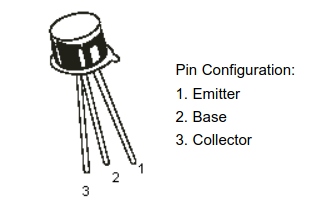
\includegraphics[width=0.5\textwidth]{bc108-pinout.png}
%   \end{center}
%   \caption{BC108 pinout}
% \end{figure}


\subsection{Biasing transistors}
\label{sec:bias}

Biasing transistors in this context means setting their
collector voltage to a certain value, while there is no
audio signal coming in.

Because Fur Face internally uses feedback for bias, you'd
have to go back and forth a couple of times between Q1 and
Q2 to make sure the voltages are right. That's because
changing the bias of one of the transistors affects the
other.

Here's the biasing procedure:

\begin{itemize}
  \item Set your multimeter up for measuring DC voltage.
    We'll be measuring values between \SI{0}{\V} and
    \SI{9}{\V};

  \item Clip or touch the black (ground) lead of the
    multimeter to any ground point in the circuit. For
    example the lug on the audio jacks that's connected via
    a black wire to GND on the PCB;

  \item Starting with transistor Q2, then moving to Q1, then
    back and forth between the two a couple of times:

    \begin{itemize}
      \item Clip or touch the red (hot) lead of the
        multimeter to the collector of the transistor;

      \item Make sure you can see there's some voltage
        readout on the multimeter;

      \item With a small screwdriver twist the screw of the
        trimpot above that transistor, so that the voltage
        gets close to the desired value (Q1 to about
        \SI{1.3}{\V}, Q2 to about \SI{5.8}{\V}). The change
        is going to be slow initially, but as the voltage
        grows, the increments are going to be more and more
        significant;
    \end{itemize}

\end{itemize}

% \section{Step-by-step Instructions}
% \label{sec:steps}

\section{Schematic}
\label{sec:schematic}

% \begin{figure}[h!]
%   \centering
%   \includegraphics[width=2\textwidth, trim={0 4cm 0cm 0cm}, page=2, clip, angle=-90]{schem.pdf}
% \end{figure}

\newgeometry{}
\restoregeometry{}

\begin{versionhistory}
  \vhEntry{1.0}{Apr 25, 2025}{AS}{Created}
\end{versionhistory}

\end{document}
